\chapter{Metodologia}
\label{cap:metodologia}

\section{Implementação do Curriculum Learning}

\subsection{Inspiração para modelagem do curriculum}

A modelagem do curriculum foi inspirada em casos reais de jogos eletrônicos populares que implementam sistemas de treinamento progressivo. Jogos como FIFA e Rocket League possuem seções dedicadas ao treinamento que seguem uma abordagem gradual de aprendizado, muito similar aos conceitos fundamentais do Curriculum Learning. No FIFA, por exemplo, o jogador começa aprendendo habilidades básicas como passes, chutes e dribles isoladamente, antes de progredir para situações mais complexas de jogo. De forma análoga, no Rocket League, os jogadores são introduzidos primeiro aos controles básicos do carro, como aceleração e saltos, evoluindo gradualmente para manobras aéreas e jogadas táticas elaboradas. Esta progressão natural do aprendizado, onde conceitos fundamentais são dominados antes da exposição a cenários mais desafiadores, alinha-se perfeitamente com os princípios do Curriculum Learning. A técnica propõe justamente esta abordagem estruturada, onde o agente é exposto a tarefas progressivamente mais complexas, permitindo que construa uma base sólida de conhecimento antes de enfrentar situações que exigem a combinação de múltiplas habilidades. Esta inspiração nos levou a modelar nosso curriculum de forma similar, começando com fundamentos básicos do futebol de robôs e progressivamente introduzindo cenários mais desafiadores e complexos.

\subsection{Isolamento e classificação de tarefas}

O processo de isolamento e classificação das tarefas foi estruturado em três níveis progressivos de complexidade, implementados através da classe \texttt{SSLCurriculumEnv}:

\begin{enumerate}
    \item \textbf{Nível 0 - Posições Fixas:} 
    \begin{itemize}
        \item Bola posicionada em coordenadas fixas (1.0, 1.0)
        \item Robô posicionado em coordenadas fixas (-1.0, -1.0)
        \item Ambiente previsível para aprendizado inicial
    \end{itemize}

    \item \textbf{Nível 1 - Posições Aleatórias:}
    \begin{itemize}
        \item Bola e robô posicionados aleatoriamente no intervalo [-2, 2]
        \item Introduz variabilidade nas condições iniciais
        \item Força o agente a generalizar seu comportamento
    \end{itemize}

    \item \textbf{Nível 2 - Obstáculos:}
    \begin{itemize}
        \item Mantém posições aleatórias do nível anterior
        \item Adiciona um obstáculo entre o robô e a bola
        \item Obstáculo posicionado a 50\% da distância entre robô e bola
    \end{itemize}
\end{enumerate}

\subsection{Modularização dos algoritmos de aprendizagem}

A modularização do aprendizado foi implementada através do \texttt{CurriculumCallback}, que gerencia a progressão entre os níveis de dificuldade. Os principais componentes são:

\begin{itemize}
    \item \textbf{Histórico de Sucesso:} Mantém registro do desempenho do agente nas últimas tentativas

    \item \textbf{Critérios de Progressão:}
    \begin{itemize}
        \item Taxa de sucesso calculada sobre uma janela de avaliação configurável
        \item Progride quando atinge limiar de promoção pré-definido
        \item Atualização automática do nível de tarefa em todos os ambientes
    \end{itemize}

    \item \textbf{Sistema de Recompensas Adaptativo:}
    \begin{itemize}
        \item Recompensa base do ambiente
        \item Penalização proporcional à distância até a bola
        \item Penalização por tempo para incentivar eficiência
        \item Penalização adicional por colisão com obstáculos no nível 2
    \end{itemize}
\end{itemize}

\begin{figure}[H]
    \centering
    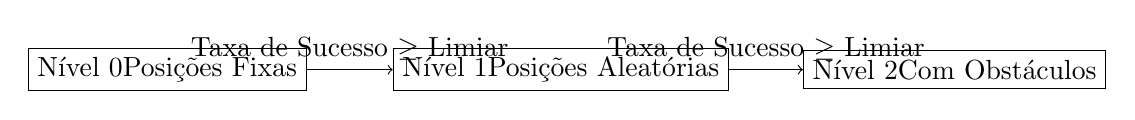
\begin{tikzpicture}[node distance=2cm]
        \node[draw,rectangle] (n0) {Nível 0\\Posições Fixas};
        \node[draw,rectangle,right of=n0,xshift=3cm] (n1) {Nível 1\\Posições Aleatórias};
        \node[draw,rectangle,right of=n1,xshift=3cm] (n2) {Nível 2\\Com Obstáculos};
        
        \draw[->] (n0) -- node[above] {Taxa de Sucesso $\geq$ Limiar} (n1);
        \draw[->] (n1) -- node[above] {Taxa de Sucesso $\geq$ Limiar} (n2);
    \end{tikzpicture}
    \caption{Progressão do Curriculum Learning implementado}
    \label{fig:curriculum_progression}
\end{figure}



\section{Parametrização do Ambiente}

\subsection{Cenários de treinamento}

\subsection{Recompensa}
%lembrar que as recompensas são varáveis de acordo com o nível de dificuldade



\section{Pipeline de Integração e Continuidade do Treinamento}

\subsection{Adaptação ao Sistema Existente}
%adaptar ao contexto do SSL-EL

\subsection{Transição entre Modos de Treinamento}



\section{Métricas e Avaliação}

Para avaliar o desempenho do agente durante o treinamento, implementamos as seguintes métricas:

\begin{itemize}
    \item \textbf{Taxa de Sucesso:} Percentual de conclusão bem-sucedida das tarefas
    \item \textbf{Tempo de Conclusão:} Duração média para completar cada tarefa
    \item \textbf{Eficiência de Trajetória:} Razão entre o caminho ideal e o realizado
    \item \textbf{Robustez:} Capacidade de manter o desempenho sob perturbações
\end{itemize}

O monitoramento destas métricas é realizado continuamente através de um sistema automatizado de coleta e análise de dados.